\documentclass[polish,12pt]{aghthesis}
\usepackage[utf8x]{inputenc}
\usepackage{url}
\usepackage{graphicx}
\usepackage{hyperref}

\graphicspath{ {./images/} }

\author{Piotr Szczygieł}

\titlePL{Gra typu Capture-The-Flag\\ oparta o reverse engineering}
\titleEN{Capture-The-Flag game based on reverse engineering}

\fieldofstudy{Informatyka}

\supervisor{dr inż.\ Łukasz Faber}

\date{\the\year}

\begin{document}

\maketitle

\section{\SectionTitleProjectVision}
\label{sec:cel-wizja}

Gra typu Capture-the-Flag jest to rodzaj zawodów z ogólnie pojętego
bezpieczeństwa komputerowego. Ich celem zwykle jest edukacja uczestników
o zabezpieczeniach systemów oraz możliwość pokazania im jak reagować
na wypadek wystąpienia rzeczywistych ataków. Zawody takie podzielone są zazwyczaj
na poszczególne zadania z różnych kategorii. Aby rozwiązać takie zadanie należy
znaleźć "flagę", którą następnie podaje się w interfejsie udostępnionym przez
organizatora zawodów. Flagą w tym wypadku jest ciąg znaków, który możemy uzyskać
poprzez rozwiązanie zadania. Przykładowo w najprostszych zadaniach
z dziedziny eksploitacji stron internetowych, flagę możemy znaleźć klikając
"Pokaż źródło strony" w przeglądarce internetowej.

\begin{figure}[h]
    \centering
    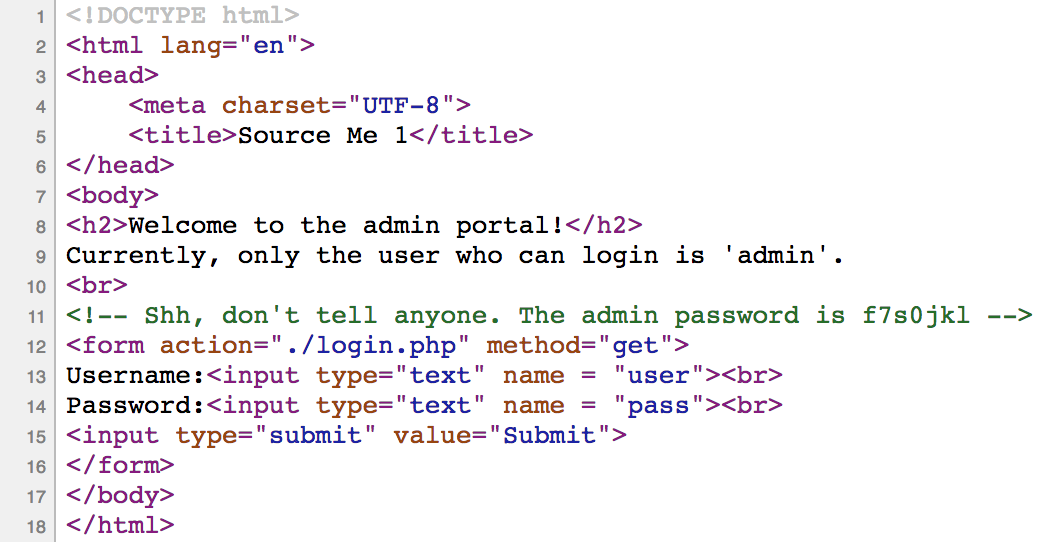
\includegraphics[width=10cm]{flag_page_source}
    \caption{Flaga \textbf{f7s0jkl} ukryta w źródle strony internetowej}
    \label{fig:flag_page_source}
\end{figure}

W mojej pracy będę prezentował jednak grę opartą
wyłącznie o Reverse Engineering (ang. Inżynieria Wsteczna).
Inżynieria wsteczna oprogramowania może odbywać się na różne sposoby.
Może to być przykładowo wykorzystanie tzw. snifferów do analizy protokołów
komunikacyjnych aplikacji internetowej. W naszym wypadku będzie ona jednak
zazwyczaj oznaczała proces analizy programu, aby zrozumieć co robi
oraz w jaki sposób. Zadania, które przedstawię można by też podpiąć do kategorii
eksploitacji binarnej (ang. Binary Exploitation), która w pewny sposób pokrywa
się z zagadnieniami Reverse Engineeringu. Jest to mianowicie proces
wykorzystywania niedoskonałości programów w celu zmuszenia ich do zrobienia
czegoś, czego w normalnej sytuacji nie powinny robić. Te dwie kategorie pokrywają
się ze sobą, ponieważ zazwyczaj nie jest możliwe rozwiązanie zadania z kategorii
eksploitacji binarnej, bez wykorzystania do tego inżynierii wstecznej. \pagebreak

Produktem końcowym będzie zbiór kilku zadań udostępniony na platformie webowej.
Platforma sama w sobie nie jest niczym specjalnym, udostępnia jedynie takie powszechne
funkcjonalności jak rejestracja użytkowników, ranking najlepszych graczy,
pobieranie zadań oraz interfejs umożliwiający wprowadzanie znalezionych
flag. Z tego względu użyję już gotowej platformy \href{https://ctfd.io}{CTFd}.
Użycie takiego gotowego rozwiązania pozwoli mi w pełni skupić się na samych zadaniach
i nie przejmować się takimi rzeczami jak gracze próbujący łamać zabezpieczenia
platformy.

\begin{figure}[h]
    \centering
    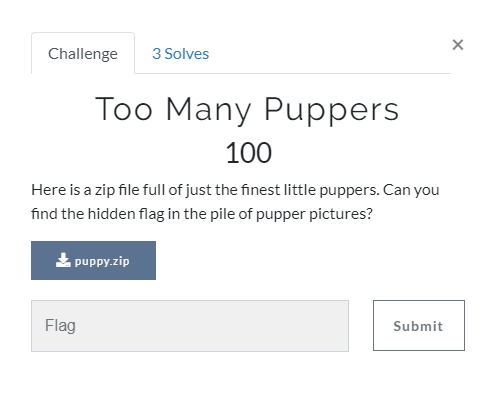
\includegraphics[width=10cm]{ctfd}
    \caption{Przykładowe zadanie na stronie demonstracyjnej CTFd}
    \label{fig:ctfd}
\end{figure}

W tej pracy opisze zarówno proces tworzenia poszczególnych zadań,
jak i przykładowe ich rozwiązania. Używam słowa "przykładowe", ponieważ
w takiej kategorii jak Binary Exploitation / Reverse Engineering liczba sposobów
na rozwiązanie danego zadania jest ograniczona jedynie przez wyobraźnie uczestnika.
Nie będę się również ograniczał do korzystania ciągle z tych samych narzędzi.
Postaram się pokazać różnorodne podejścia do analizy i rozwiązywania wyzwań.
Zadania będą tworzone z zamiarem zachowania rosnącego stopnia trudności.
Na początku uczestnik będzie miał szansę rozwiązać proste zadania,
zachęcające go do dalszej rozgrywki. Finalne zadania powinny stanowić wyzwanie
nawet dla doświadczonych graczy. \pagebreak

Aktualnie istnieje wiele różnych zawodów CTF online.
Jednym z popularniejszych jest \newline \href{https://picoctf.com}{picoCTF}.
Można tam kiedykolwiek wejść, zalogować się i zająć się rozwiązywaniem problemów.

\begin{figure}[h]
    \centering
    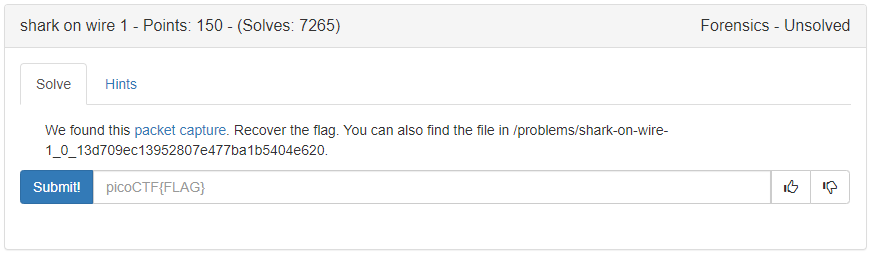
\includegraphics[width=10cm]{picoctf}
    \caption{Zadanie z kategorii Forensics na stronie picoCTF}
    \label{fig:picoctf}
\end{figure}

Moją główną motywacją jednak jest fakt, że strony tego typu często skupiają
się na zadaniach w takich kategoriach jak Forensics czy Web Exploitation.
Mnie natomiast bardzo interesuję temat inżynierii wstecznej i chciałem
przygotować wyzwania oparte o zadania tylko z tej kategorii.

Zadania będą tworzone w języku C. Jest to powszechnie znany język, który
z wyłączoną zbyt agresywną optymalizacją ze strony kompilatora, generuje
w miarę przewidywalny kod maszynowy. Zaletą tego jest to, że narzędzia
do debugowania, dezasemblacji oraz wykonywania innych analiz programów
bardzo dobrze radzą sobie z takimi plikami. Dzięki temu język ten
zapewni nam kontrolę nad tym w jakim stopniu graczowi ułatwimy
lub utrudnimy rozgrywkę. W celu zapewnienia większej różnorodności
środowisk korzystać będziemy zarówno z systemu Windows jak i Linux.

Do rozwiązywania zadań posłużymy się różnorodnymi rodzajami narzędzi.
Poczynając od linuxowych programów linii poleceń takich jak \emph{strings}
czy \emph{gdb}, pisania własnych narzędzi w języku \emph{Python},
czy w końcu korzystając z pełnoprawnych narzędzi z interfejsem graficznym takich
jak używana przez NSA \emph{Ghidra}, czy debugger dla systemu
Windows \emph{RemedyBG}.

\clearpage

%\emph{Charakterystyka problemu, motywacja projektu (w tym przegląd
%  istniejących rozwiązań prowadząca do uzasadnienia celu prac),
%  wizja produktu i analiza zagrożeń.}

\section{\SectionTitleScope}
\label{sec:zakres-funkcjonalnosci}
%\emph{Kontekst użytkowania produktu (aktorzy, współpracujące systemy)
%  oraz specyfikacja wymagań funkcjonalnych i niefunkcjonalnych.}

\section{\SectionTitleRealizationAspects}
\label{sec:wybrane-aspekty-realizacji}
% \emph{Przyjęte założenia, struktura i zasada działania systemu,
%   wykorzystane rozwiązania technologiczne wraz z uzasadnieniem
%   ich wyboru, istotne mechanizmy i zastosowane algorytmy.}

\section{\SectionTitleWorkOrganization}
\label{sec:organizacja-pracy}
% \emph{Struktura zespołu (role poszczególnych osób), krótki opis i
%   uzasadnienie przyjętej metodyki i/lub kolejności prac, planowane i
%   zrealizowane etapy prac ze wskazaniem udziału poszczególnych
%   członków zespołu, wykorzystane praktyki i narzędzia w zarządzaniu
%   projektem.}

\section{\SectionTitleResults}
\label{sec:wyniki-projektu}
% \emph{Wskazanie wyników projektu (co konkretnie udało się uzyskać:
%   oprogramowanie, dokumentacja, raporty z testów/wdrożenia, itd.), prezentacja wyników
%   i ocena ich użyteczności (jak zostało to zweryfikowane --- np.\ wnioski
%   klienta/użytkownika, zrealizowane testy wydajnościowe, itd.),
%   istniejące ograniczenia i propozycje dalszych prac.}

% o ile to możliwe proszę używać odwołań \cite w konkretnych miejscach a nie \nocite

% \nocite{artykul2011,ksiazka2011,narzedzie2011,projekt2011}

% \bibliography{bibliography}

\end{document}
